\chapter{Results and Discussion}

\section{Motor Movement}
Due to the high objectivity of brain activity due to motor movement, measuring brain activity due to motor movement is perhaps the best way to asses the system. Placing the sensor above the top left motor cortex (refer to Figure 5.1), and having the test subject do the 'chicken dance' (that is repeatably touching the thumb to the tip of each finger) with their right hand for 30s yields the results in Figure 5.2. Note that the subject started the 'chicken dance' at around 1s, stopped movement to see the effect, then resumed the chicken dance again, and then finally stopped movement before the end of the test.

\begin{figure}[htp]
\centering
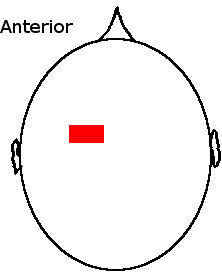
\includegraphics[width=2in]{motorsens.png}
\caption[Placement of Sensor to Measure Right Hand Movement]{Approximate placement of the sensor to measure right hand movement. The sensor, marked in red, is positioned above the left motor cortex.}
\end{figure}

\begin{figure}[htp]
\centering
\subfigure[Sensor 1]{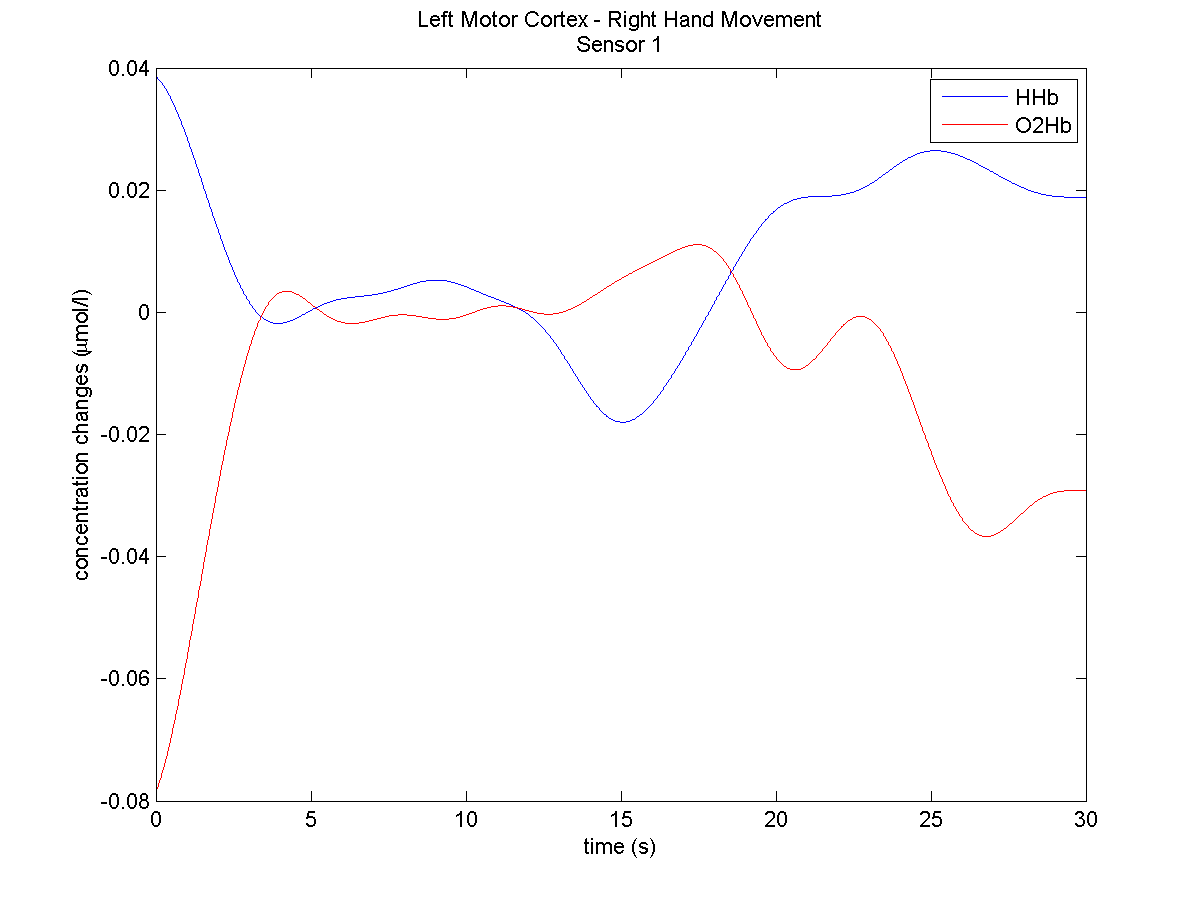
\includegraphics[width=4in]{LeftMotorCortex-RightHandMovement/sensor1.png}}
\subfigure[Sensor 2]{ 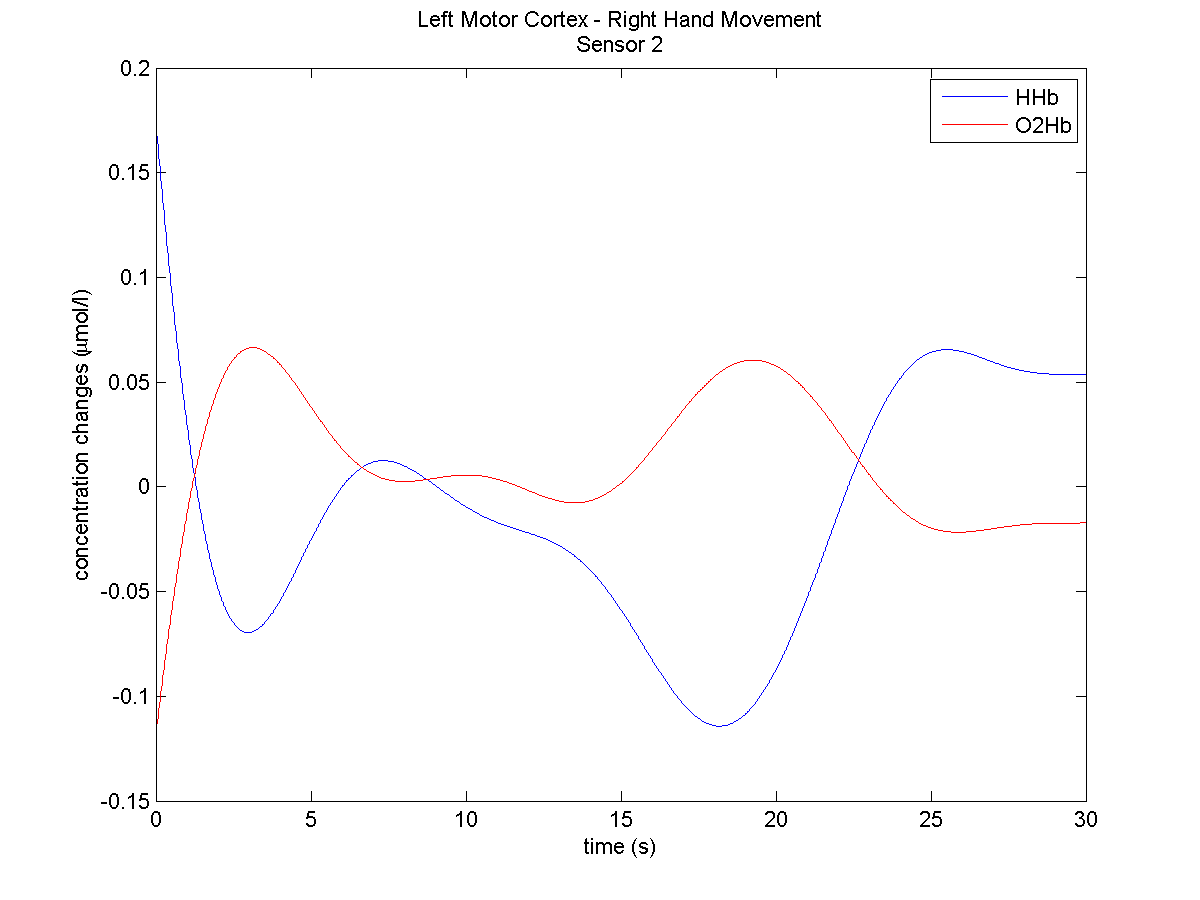
\includegraphics[width=4in]{LeftMotorCortex-RightHandMovement/sensor2.png}}
\caption[Left Motor Cortex Measurements with Motor Movement]{The result of having the subject move their right hand with the sensor placed over the left motor cortex. The change in concentration of oxyhaemoglobin is marked in red and the change in concentration of deoxyhaemoglobin is marked in blue. The subject began the 'chicken dance' at ~1s, briefly stopped at around 7s, started the 'chicken dance' again at around 9s, and finally stopped at around 22s, as can be seen in the Sensor 2 measurements.}
\end{figure}

The measurements from Sensor 1 do not seem to be correct. It is excessively noisy, masking the haemodynamic effect of the blood perfusion that is the result of the motor movement. Perhaps, the photodiode is damaged or the lens scratched/dirty. There was not enough time to correctly trouble shoot the problem. In either case, the results from Sensor1, while it does pick up varying light intensities, contains too much noise to extract the relevant data from it. As such, the results from Sensor 1 should be ignored. However, for the sake of completeness and to correctly asses the system, figures of the measurements from Sensor 1 will still be included, though not discussed. 

Looking at the figures, it can be seen that the concentration changes at the start of the measurements, while relevant, are much larger compared to the rest. This is a result of initially measuring the system from 0, thus there is a high concentration change from the beginning. Once the correct base level is achieved, the results normalize and the exact concentration changes can be seen. Therefore, when looking at the results one can safely ignore the first few measurements. One thing to note about these measurements is that the subject had long dark hair, which will decrease the overall SNR of the system.

Analyzing at the results from Sensor 2, it can be seen that with motor activity on the right part of the body, there is an increased amount of oxyhaemoglobin concentration and a decreased amount of deoxyhaemoglobin concentration. When motor activity stops (at around 7s), the amount of oxyhaemoglobin concentration decreases and the amount of deoxyhaemoglobin concentration increases. When motor activity starts up again (at around 9s), again there is an increased amount of oxyhaemoglobin concentration and a decreased amount of deoxyhaemoglobin concentration. When the motor activity finally stops completely, the amount of oxyhaemoglobin concentration decreases and the amount of deoxyhaemoglobin concentration greatly increases. This agrees with what one would expected from neuronal activation. With neuronal activation comes an increased amount of blood perfusion, thus increased amounts of oxyhaemoglobin and decreased amount of deoxyhaemoglobin. When neuronal activation stops, blood perfusion decreases, adversely, causing decreased amounts of oxyhaemoglobin and increased amount of deoxyhaemoglobin. This also agrees with the results obtained from other NIRS systems (refer to Chapter 2, Figures 2.2 and 2.3 specifically).

To better analyze motor movement, lets have a look at the same measurements but with no motor movement. To examine the case with no motor movement, the sensor was placed in roughly the same place as in Figure 5.1 with the subject attempting to stay perfectly still. The results of this are displayed in Figure 5.3.

\begin{figure}[htp]
\centering
\subfigure[Sensor 1]{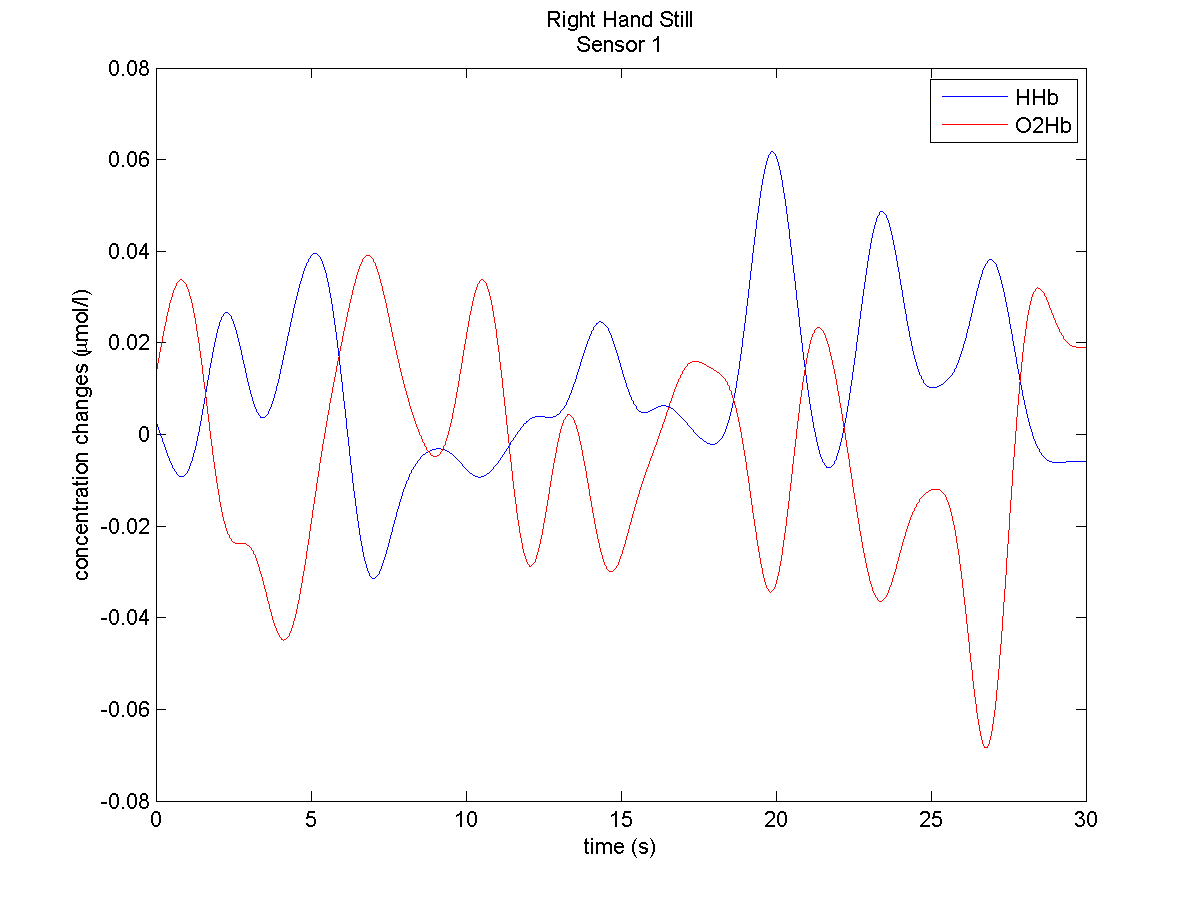
\includegraphics[width=4in]{LeftMotorCortex-NoMovement/sensor1.png}}
\subfigure[Sensor 2]{ 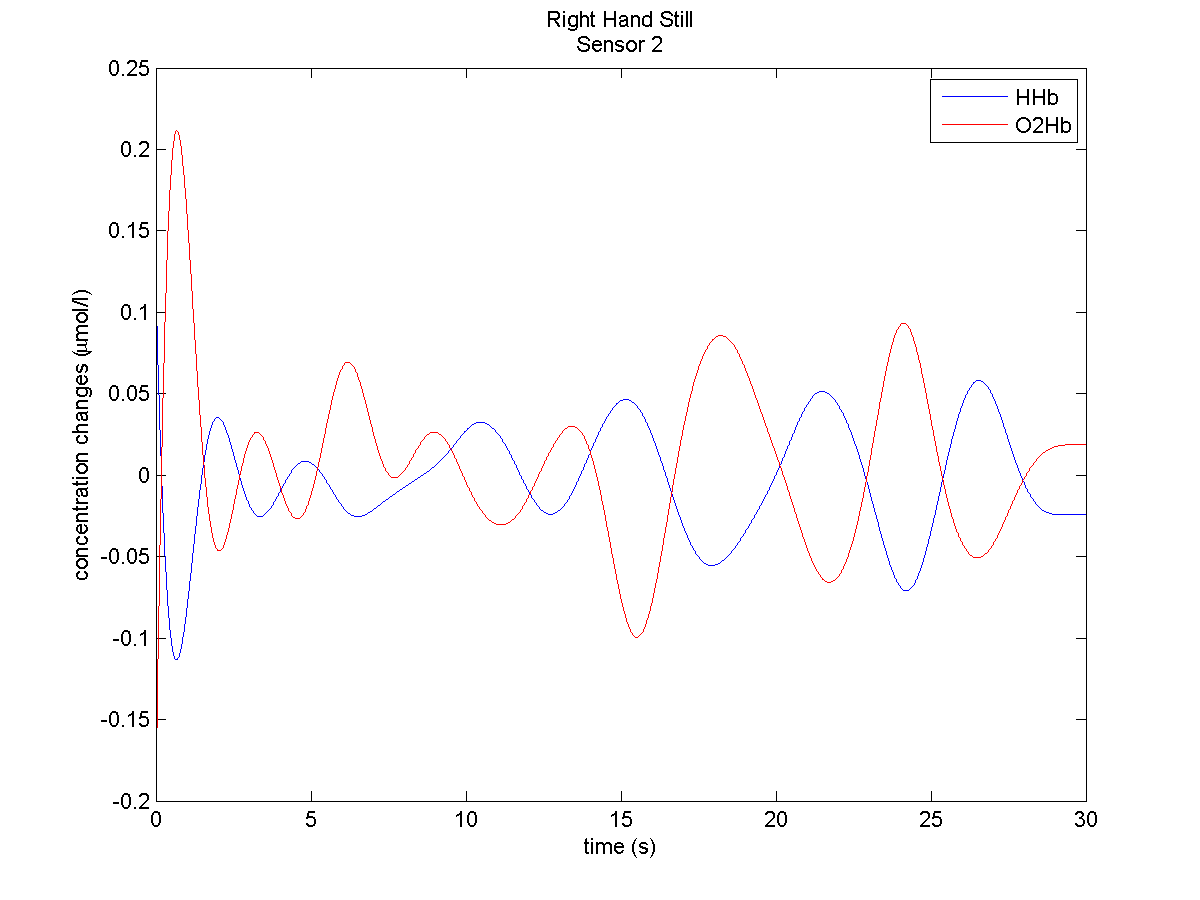
\includegraphics[width=4in]{LeftMotorCortex-NoMovement/sensor2.png}}
\caption[Left Motor Cortex Measurements with No Motor Movement]{The result of having the subject attempt to sit still with the sensor placed over the left motor cortex. The change in concentration of oxyhaemoglobin is marked in red and the change in concentration of deoxyhaemoglobin is marked in blue.}
\end{figure}

The results in Figure 5.3 show that when the subject is at rest, there is no constant increase or decrease in oxyhaemoglobin or deoxyhaemoglobin. Rather, the change in concentration constantly increases and decreases. This is probably caused by cells in the neuron consuming oxygen, increasing the deoxyhaemoglobin concentration, but with the increased level of deoxyhaemoglobin, fresh blood enters the neuron, increasing the oxyhaemoglobin concentration. With this cycle repeating itself, the results obtained would mirror that of in Figure 5.3.

To test the repeatably of this NIRS device, the same motor movement ('the chicken dance') will be done again with the sensor in roughly the same place as in Figure 5.1. It can be seen in Figure 5.4.

\begin{figure}[htp]
\centering
\subfigure[Sensor 1]{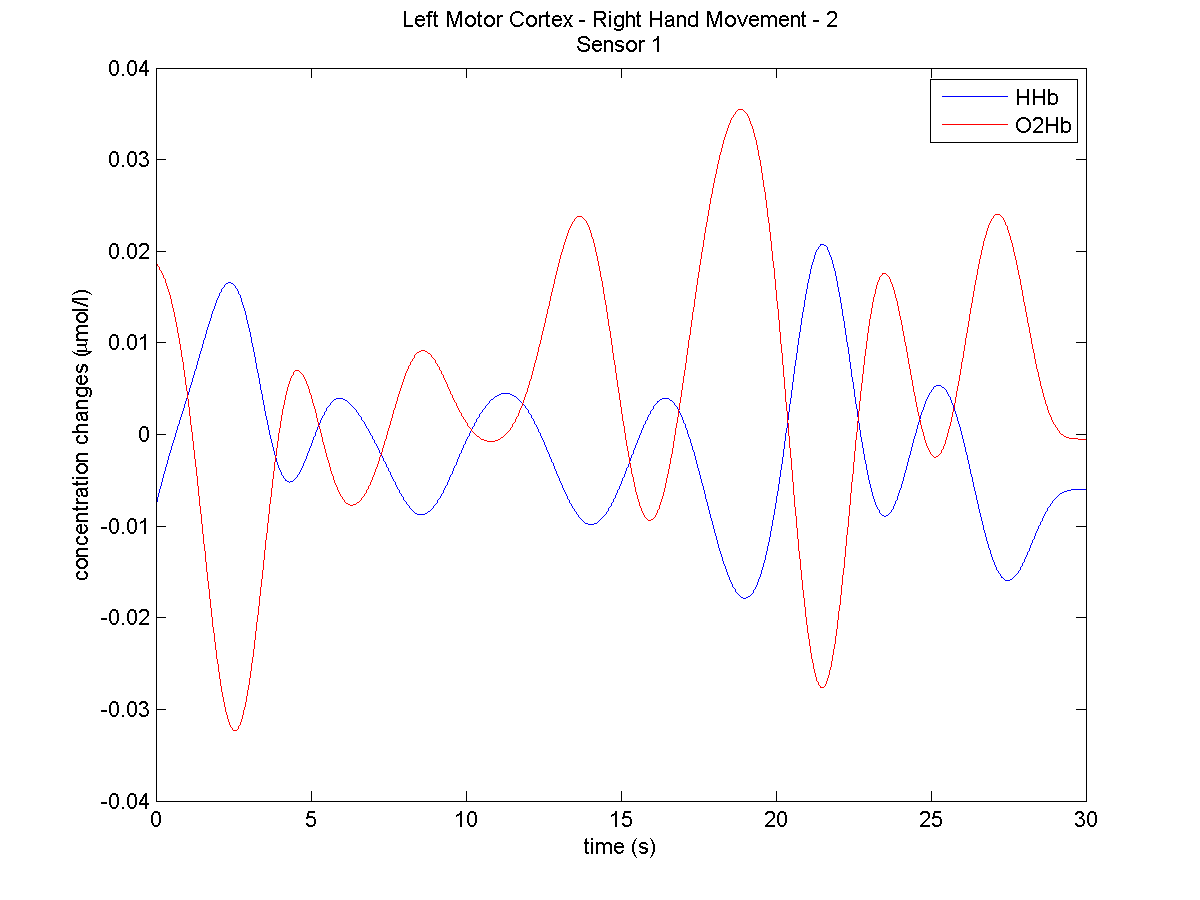
\includegraphics[width=4in]{LeftMotorCortex-RightHandMovement-2/sensor1.png}}
\subfigure[Sensor 2]{ 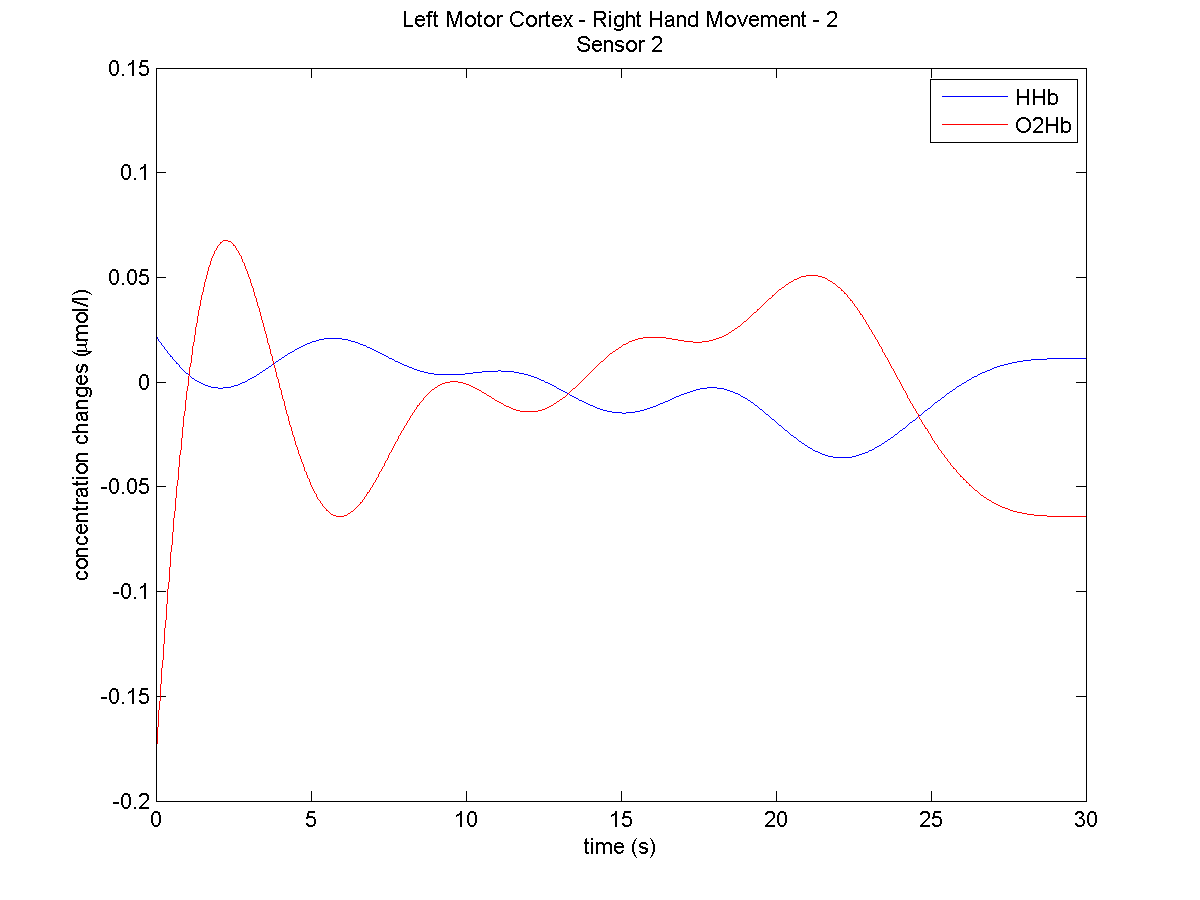
\includegraphics[width=4in]{LeftMotorCortex-RightHandMovement-2/sensor2.png}}
\caption[Left Motor Cortex Measurements with Motor Movement, Test 2]{The second result of having the subject do the 'chicken dance' with their right hand with the sensor placed over the left motor cortex. The change in concentration of oxyhaemoglobin is marked in red and the change in concentration of deoxyhaemoglobin is marked in blue. This time the subject began movement at around 0s, stopped at around 4s, and slowly began the 'chicken dance' again at around 8s before finally stopping at roughly 25s.}
\end{figure}

The results in Figure 5.4 show a good amount of repeatability. The results agree with that in the first test of right hand motor activity. When there is motor activity on the right part of the body, there is an increased amount of oxyhaemoglobin concentration and a decreased amount of deoxyhaemoglobin concentration. When the motor activity stops, the amount of oxyhaemoglobin concentration decreases and the amount of deoxyhaemoglobin concentration increases.

Doing the same test with the left hand and the sensor placed on top of the right motor cortex (refer to Figure 5.5) gives the results in Figure 5.6.

\begin{figure}[htp]
\centering
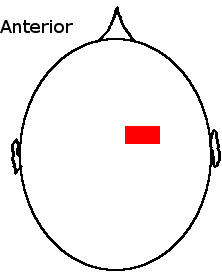
\includegraphics[width=2in]{motorsens-left.png}
\caption[Placement of Sensor to Measure Left Hand Movement]{Approximate placement of the sensor to measure left hand movement. The sensor, marked in red, is positioned above the right motor cortex.}
\end{figure}

\begin{figure}[htp]
\centering
\subfigure[Sensor 1]{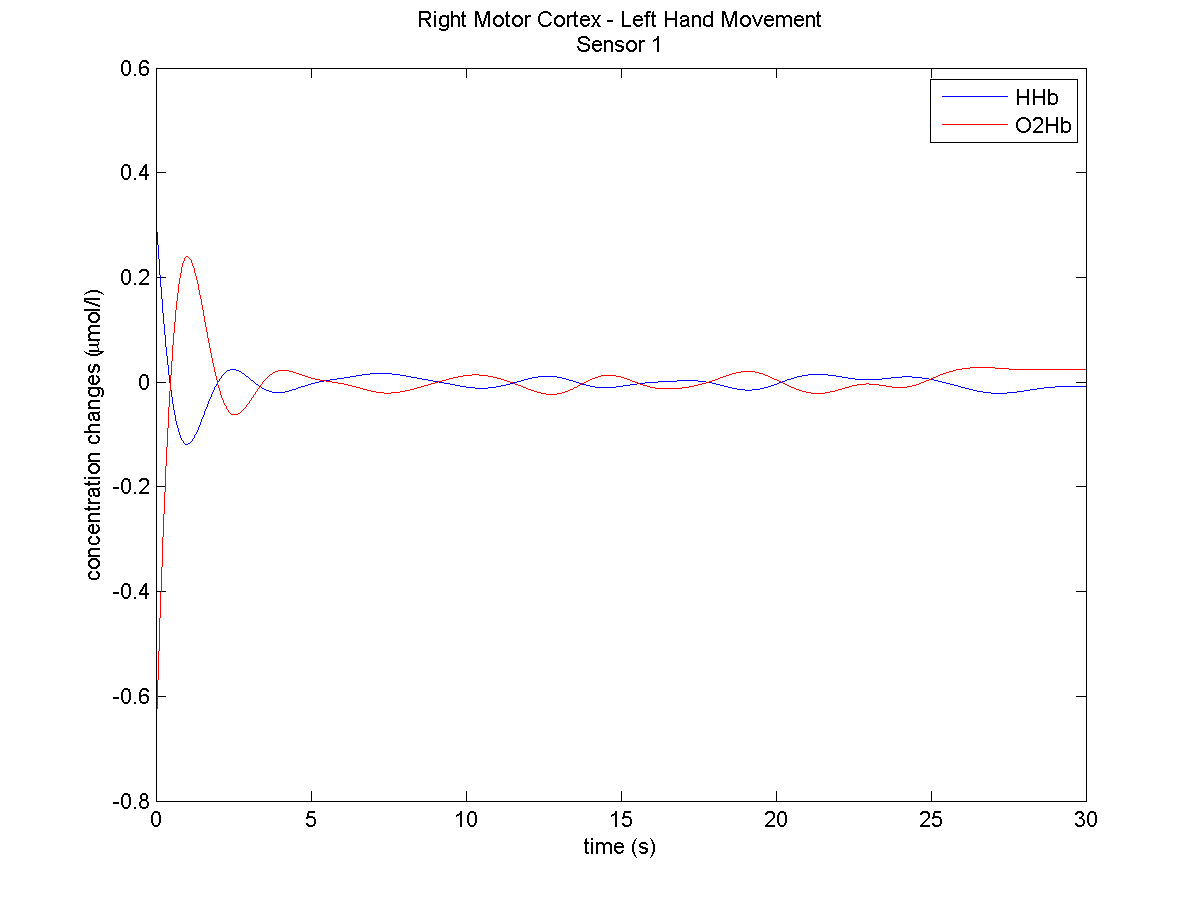
\includegraphics[width=4in]{RightMotorCortex-LeftHandMovement/sensor1.png}}
\subfigure[Sensor 2]{ 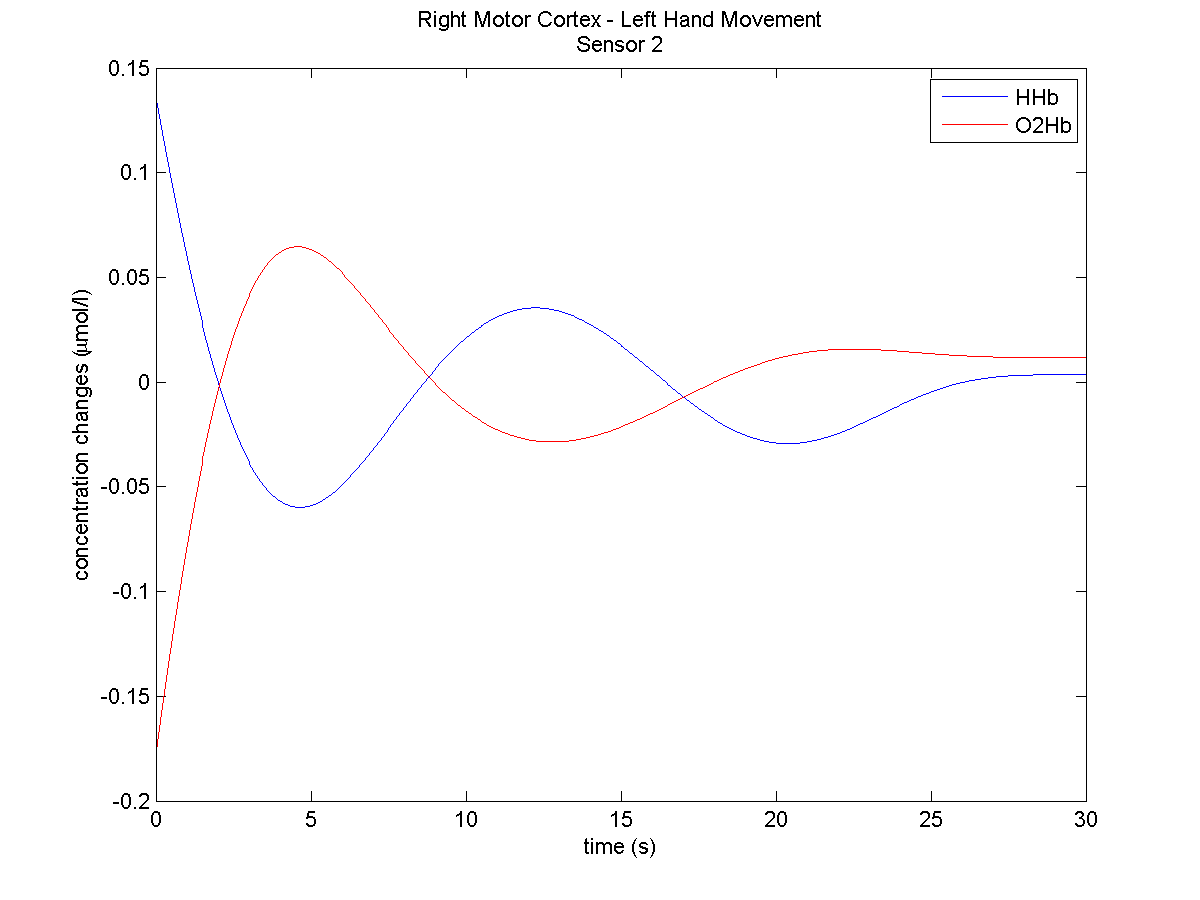
\includegraphics[width=4in]{RightMotorCortex-LeftHandMovement/sensor2.png}}
\caption[Left Motor Cortex Measurements with Motor Movement]{The result of having the subject move their left hand with the sensor placed over the right motor cortex. The change in concentration of oxyhaemoglobin is marked in red and the change in concentration of deoxyhaemoglobin is marked in blue. The subject began the 'chicken dance' at ~0s, stopped at around 7s, and started the 'chicken dance' again at around 16s, as can be seen in the Sensor 2 measurements.}
\end{figure}

Once again, it can be seen that with motor activity on the left part of the body, there is an increased amount of oxyhaemoglobin concentration and a decreased amount of deoxyhaemoglobin concentration in the right side of the motor cortex. Once more, when motor activity stops, the amount of oxyhaemoglobin concentration decreases and the amount of deoxyhaemoglobin concentration increases.

\section{Thinking Intensely}
Now that it has been shown that the NIRS device can somewhat accurately measure brain activity, others areas of the brain can be explored. Measuring brain activity in the frontal lobe while thinking about random things can be done when the sensor is placed as seen in Figure 5.7. This yields the results in Figure 5.8. Doing the same measurements but with the subject's eyes closed and in a relaxed state with the subject trying not to think about anything yields the results in Figure 5.9.

\begin{figure}[htp]
\centering
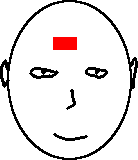
\includegraphics[width=2in]{sensorfront.png}
\caption[Placement of Sensor to measure Frontal Lobe]{Approximate placement of the sensor to measure brain activity when thinking intently. The sensor, marked in red, is positioned above the frontal lobe.}
\end{figure}

\begin{figure}[htp]
\centering
\subfigure[Sensor 1]{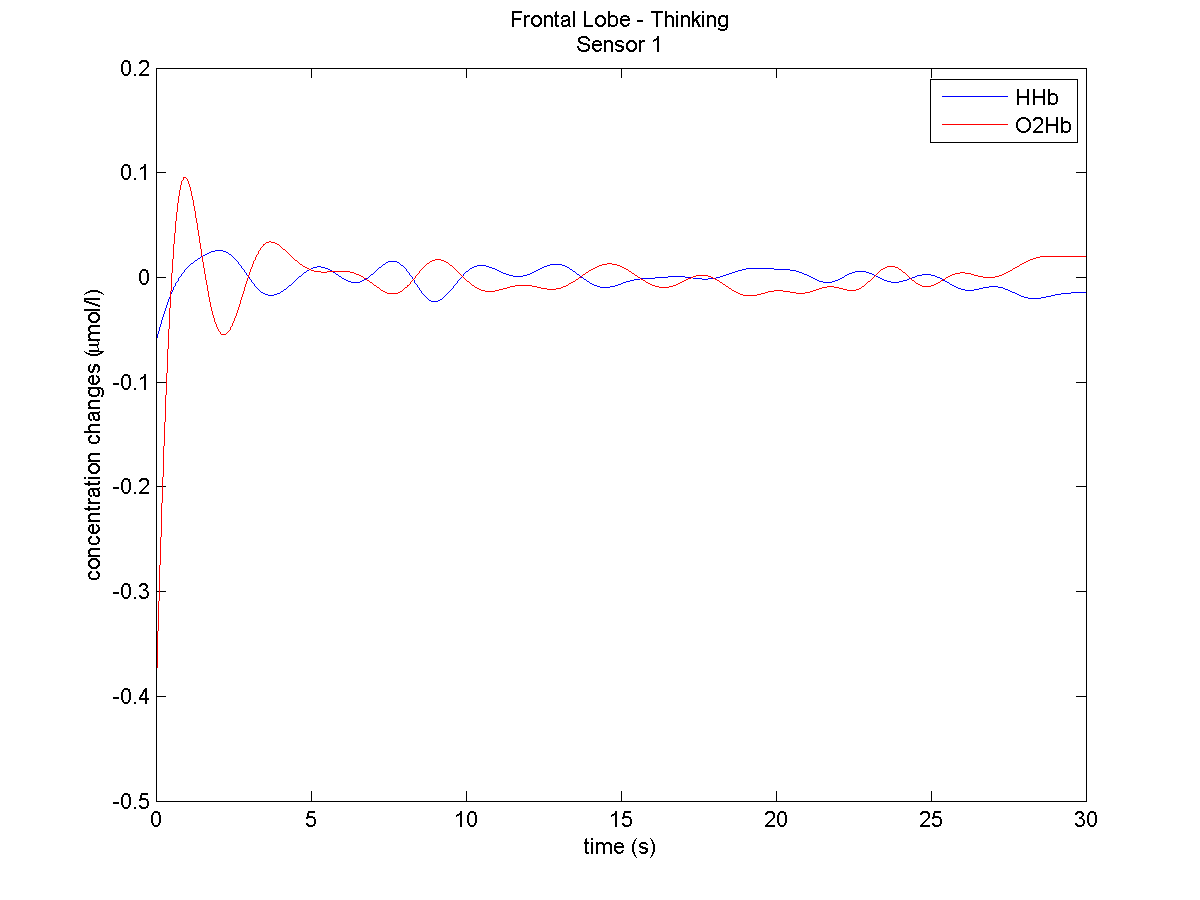
\includegraphics[width=4in]{FrontalLobe-Thinking/sensor1.png}}
\subfigure[Sensor 2]{ 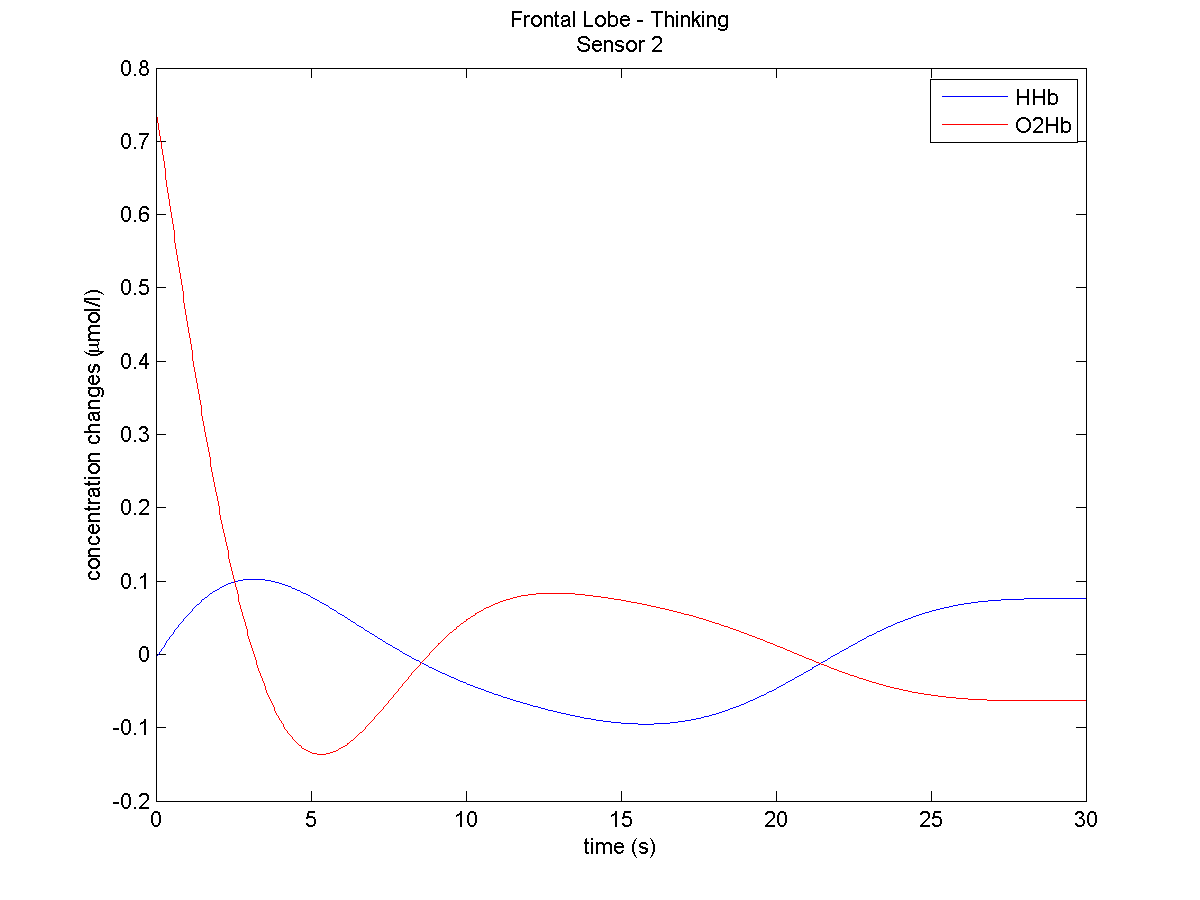
\includegraphics[width=4in]{FrontalLobe-Thinking/sensor2.png}}
\caption[Frontal Lobe Measurements while Thinking Intensely]{The result of having the subject think intensely with the sensor placed over the frontal lobe. The change in concentration of oxyhaemoglobin is marked in red and the change in concentration of deoxyhaemoglobin is marked in blue.}
\end{figure}

\begin{figure}[htp]
\centering
\subfigure[Sensor 1]{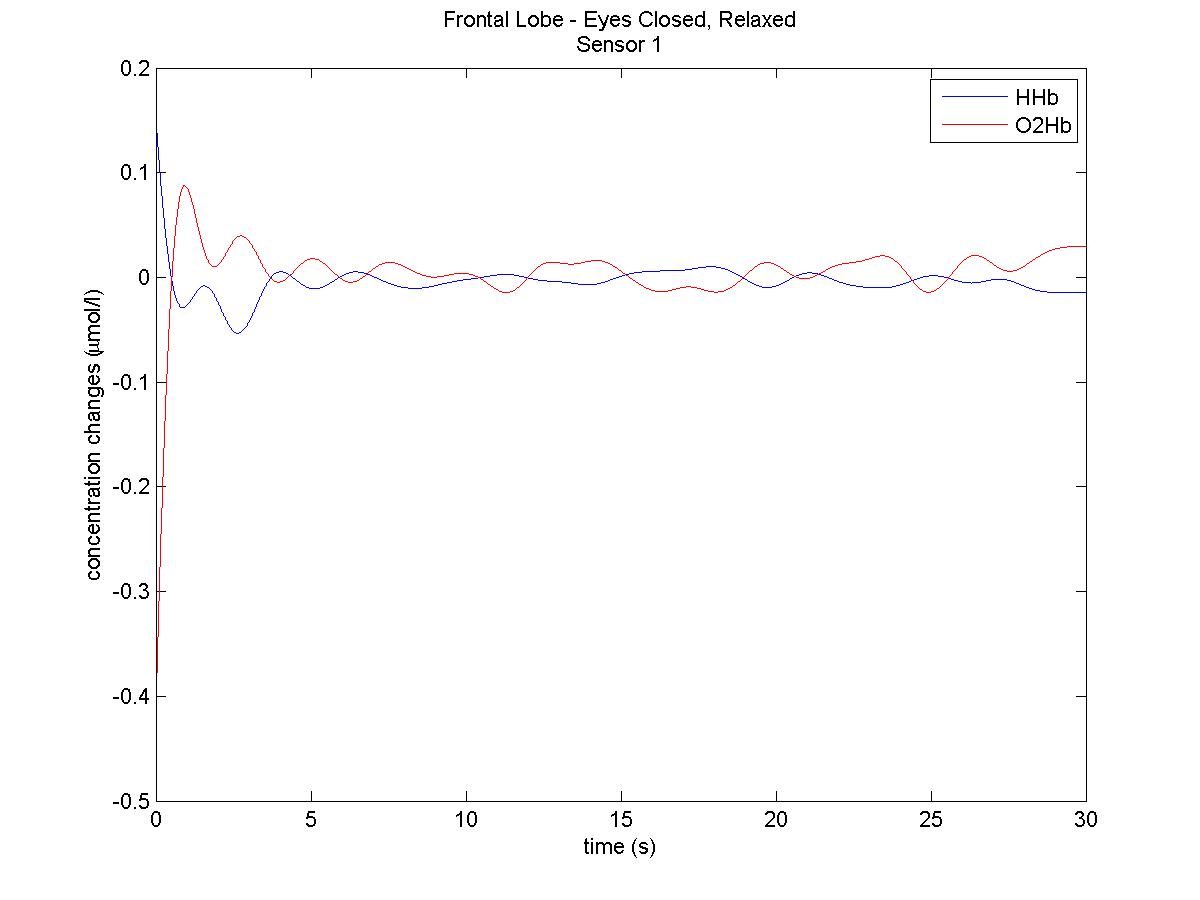
\includegraphics[width=4in]{FrontalLobe-Relaxed/sensor1.png}}
\subfigure[Sensor 2]{ 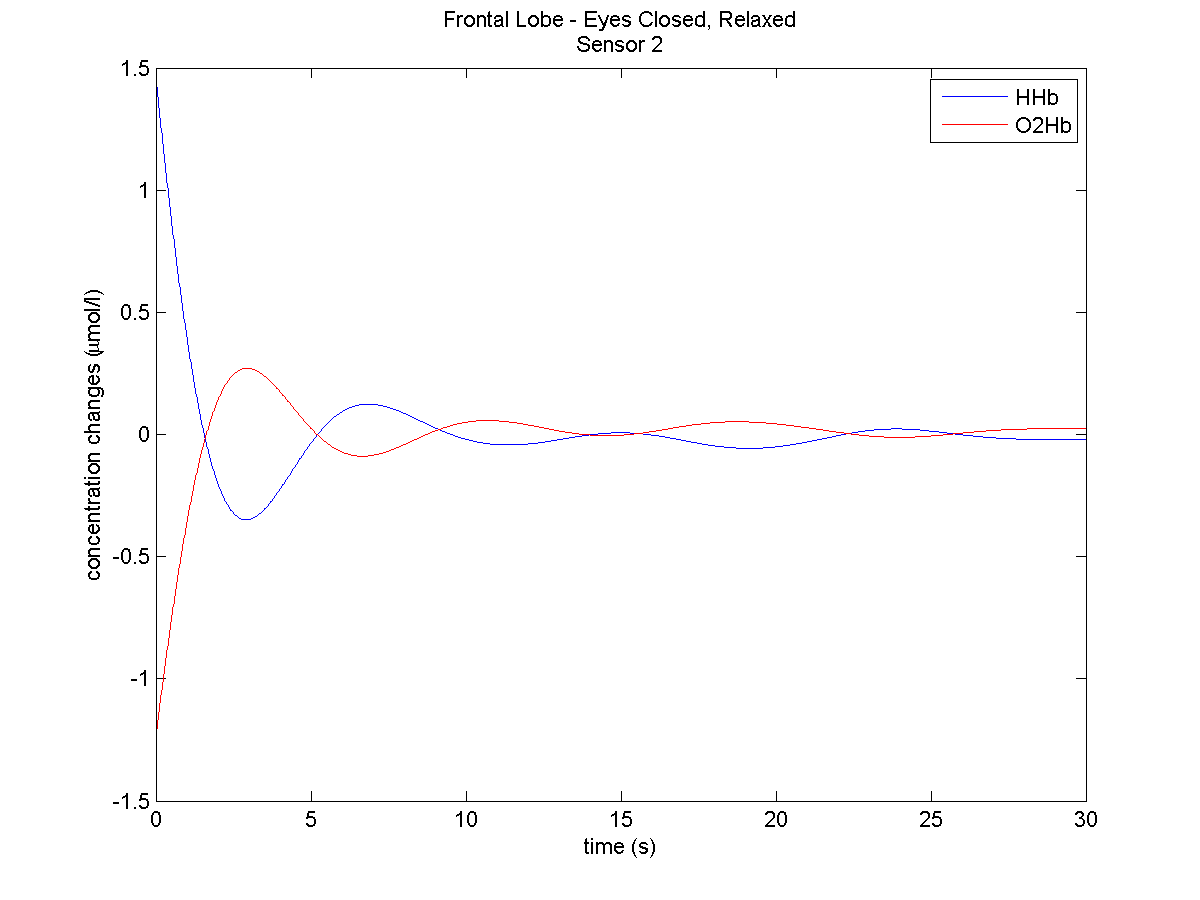
\includegraphics[width=4in]{FrontalLobe-Relaxed/sensor2.png}}
\caption[Frontal Lobe Measurements while Relaxed]{The result of having the subject not think of anything in a relaxed manor and their eyes closed with the sensor placed over the frontal lobe. The change in concentration of oxyhaemoglobin is marked in red and the change in concentration of deoxyhaemoglobin is marked in blue.}
\end{figure}

Comparing the 2 results, it can be seen that brain activity while the subject is thinking intensely can indeed by measured. When the subject is thinking intensely there is a constant increase in oxyhaemoglobin and constant decrease in deoxyhaemoglobin, showing brain activity. However, when the subject is in a relaxed non-thinking manor, the change in concentrations of oxyhaemoglobin and deoxyhaemoglobin constantly fluctuate; they are continually increases and decreasing.

\section{Visual stimulation}
Measuring the visual cortex with the subject's eyes continually moving from one intensely focused object to another, gives the results in Figure 5.11. The sensor placement can be seen in Figure 5.10. Doing the same measurements but with the subject's eye's closed, produces the result in Figure 5.12.

\begin{figure}[htp]
\centering
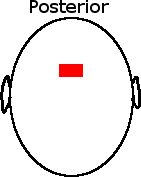
\includegraphics[width=2in]{sensorback.png}
\caption[Placement of Sensor to Measure Visual Cortex]{Approximate placement of the sensor to measure brain activity in the visual cortex. The sensor, marked in red, is positioned on top of the visual cortex.}
\end{figure}

\begin{figure}[htp]
\centering
\subfigure[Sensor 1]{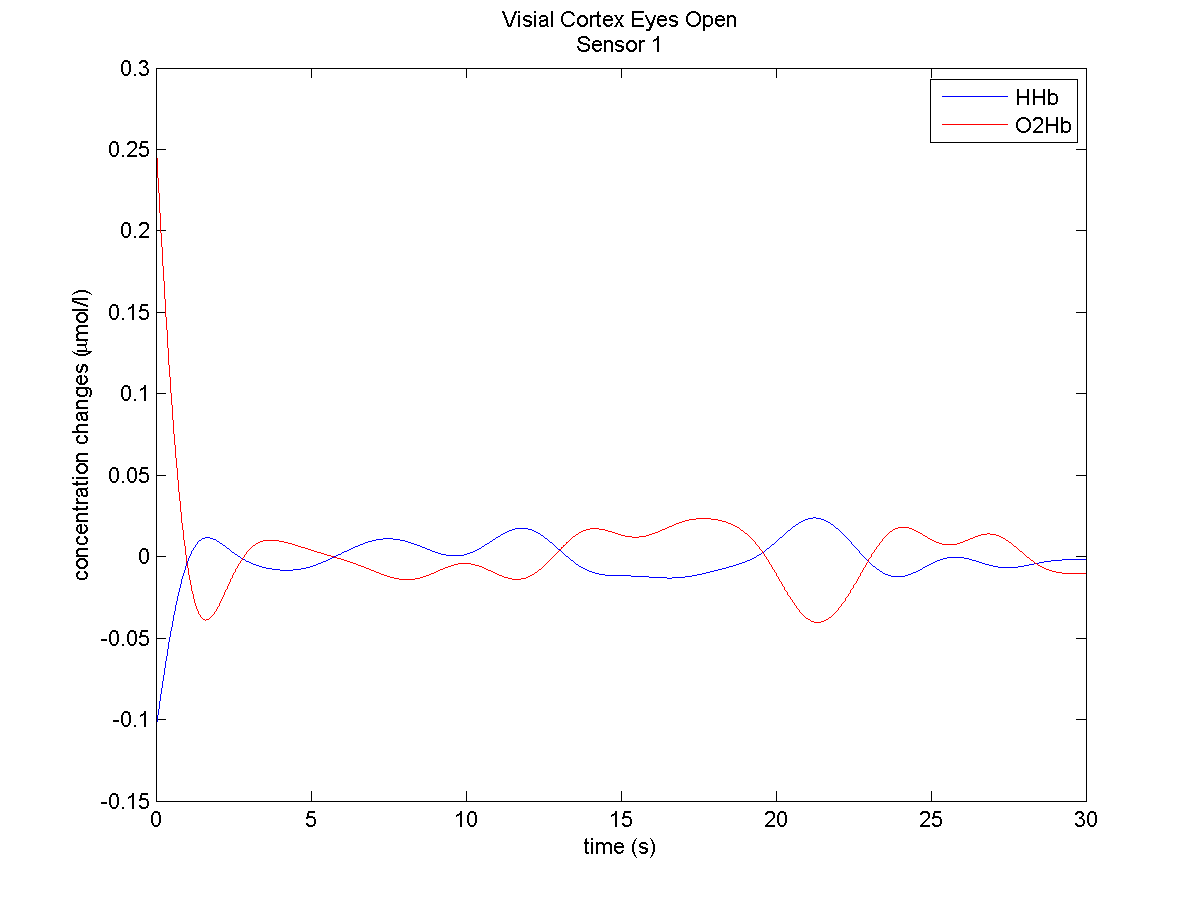
\includegraphics[width=4in]{VisialCortex-EyesOpen/sensor1.png}}
\subfigure[Sensor 2]{ 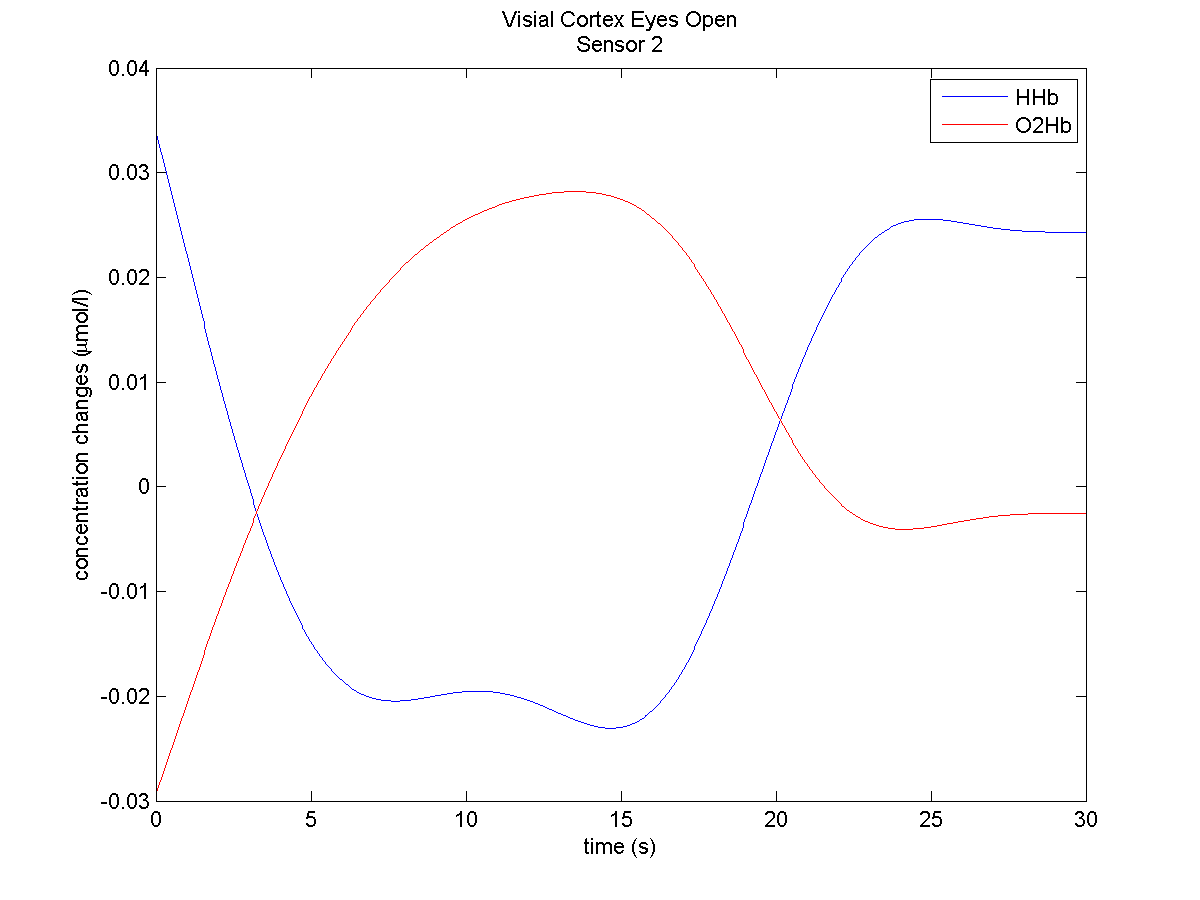
\includegraphics[width=4in]{VisialCortex-EyesOpen/sensor2.png}}
\caption[Visual Cortex Measurements while Moving Eyes between focused objects]{The result of having the subject constantly moving their eyes from different intensely focused object with the sensor placed over the visual cortex. The change in concentration of oxyhaemoglobin is marked in red and the change in concentration of deoxyhaemoglobin is marked in blue.}
\end{figure}

\begin{figure}[htp]
\centering
\subfigure[Sensor 1]{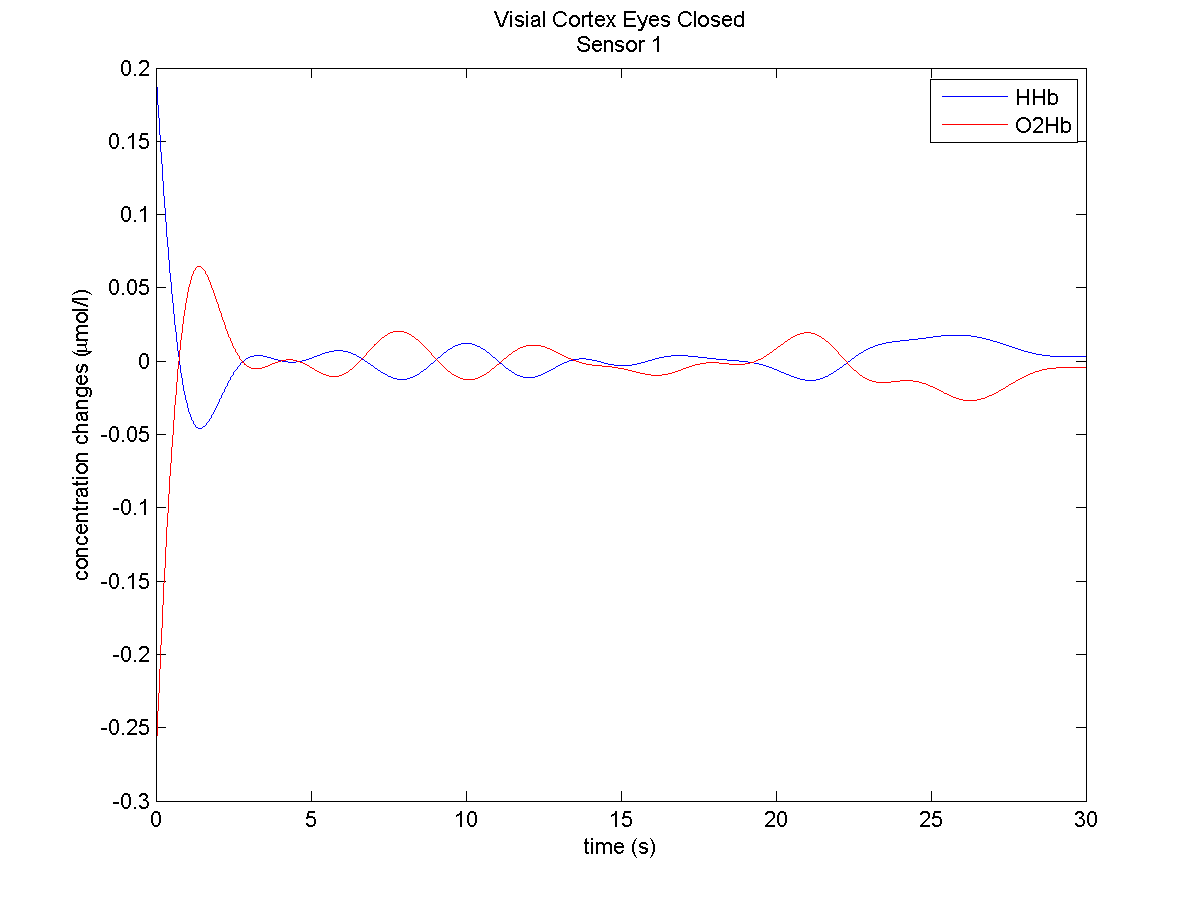
\includegraphics[width=4in]{VisialCortex-EyesClosed/sensor1.png}}
\subfigure[Sensor 2]{ 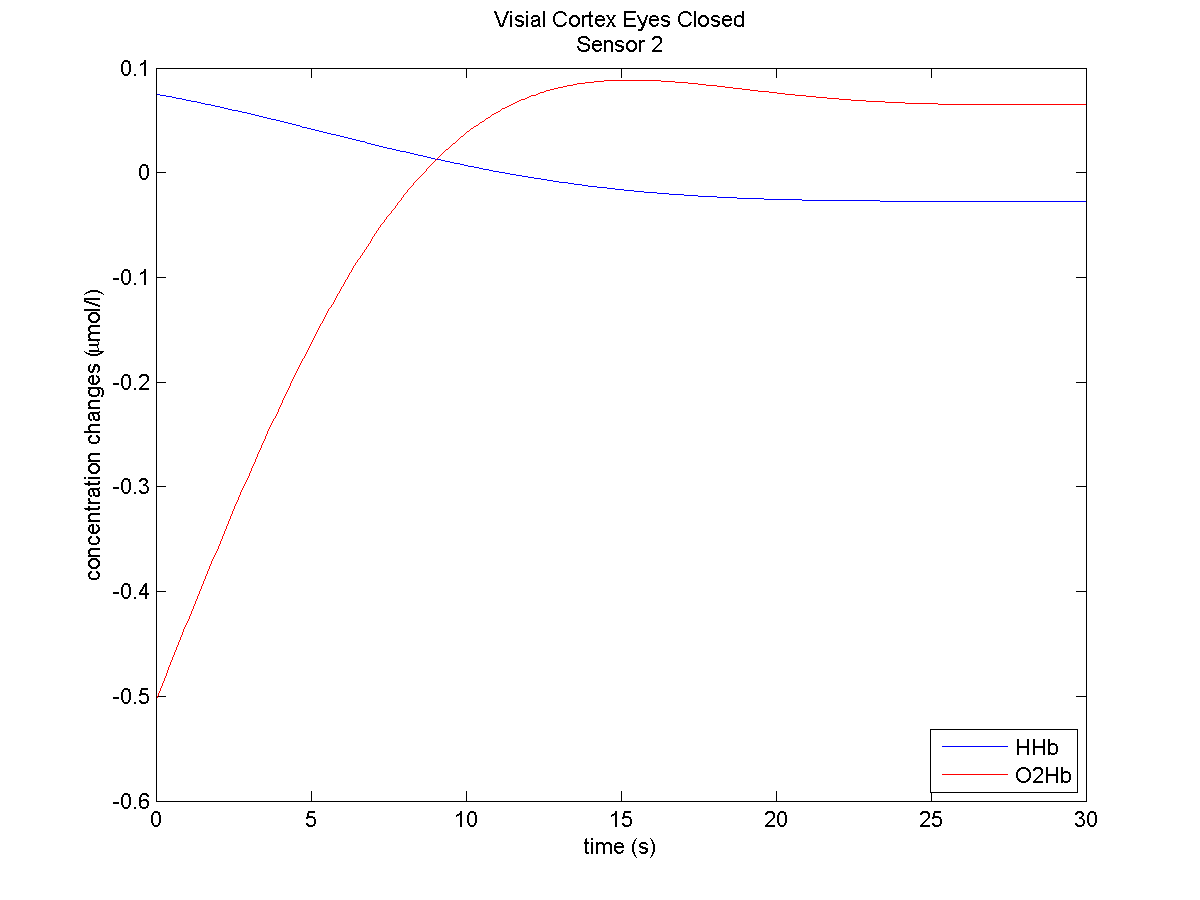
\includegraphics[width=4in]{VisialCortex-EyesClosed/sensor2.png}}
\caption[Frontal Lobe Measurements while Relaxed]{The result of having the subject close their eyes with the sensor placed over the visual cortex. The change in concentration of oxyhaemoglobin is marked in red and the change in concentration of deoxyhaemoglobin is marked in blue.}
\end{figure}

Interpreting these results is not quite clear. Even with the subject's eyes closed there seems to still be brain activity occurring in the visual cortex, though to a lesser degree than that when the subject's eyes were open. Perhaps there was movement of the sensor in the second measurements or possibly the subject was still moving their eyes with their eyes closed. 

Where the change in oxyhaemoglobin starts to increase and the change in deoxyhaemoglobin starts to increase in Figure 5.11 (with the subject's eyes open) is where the subject slowed down their eye movements and took longer to stare at each object. There is still brain activity occurring, but to a lesser degree than when the subject's eyes were moving fast, which is why there is a decrease in the change of oxygenation. This is a potential fatal flaw of this system. At this point it appears as if the subject closed their eyes or rather brain activity stopped occurring in this area. However, this was not the case, instead lower amount of oxygenation was required by the neuron. This is where a system that can exactly quantify the concentration would stand out from this system.

\section{Muscle Contractions}

As an addition to this project, the system was tested to see if it could measure muscle activity. Placing the sensor onto the test subject's bicep and having them continually flex and extend their bicep yields the result in Figure 5.13. Giving the subject a heavy weight and having them flex and extend their bicep again yields the result in Figure 5.14.

\begin{figure}[htp]
\centering
\subfigure[Sensor 1]{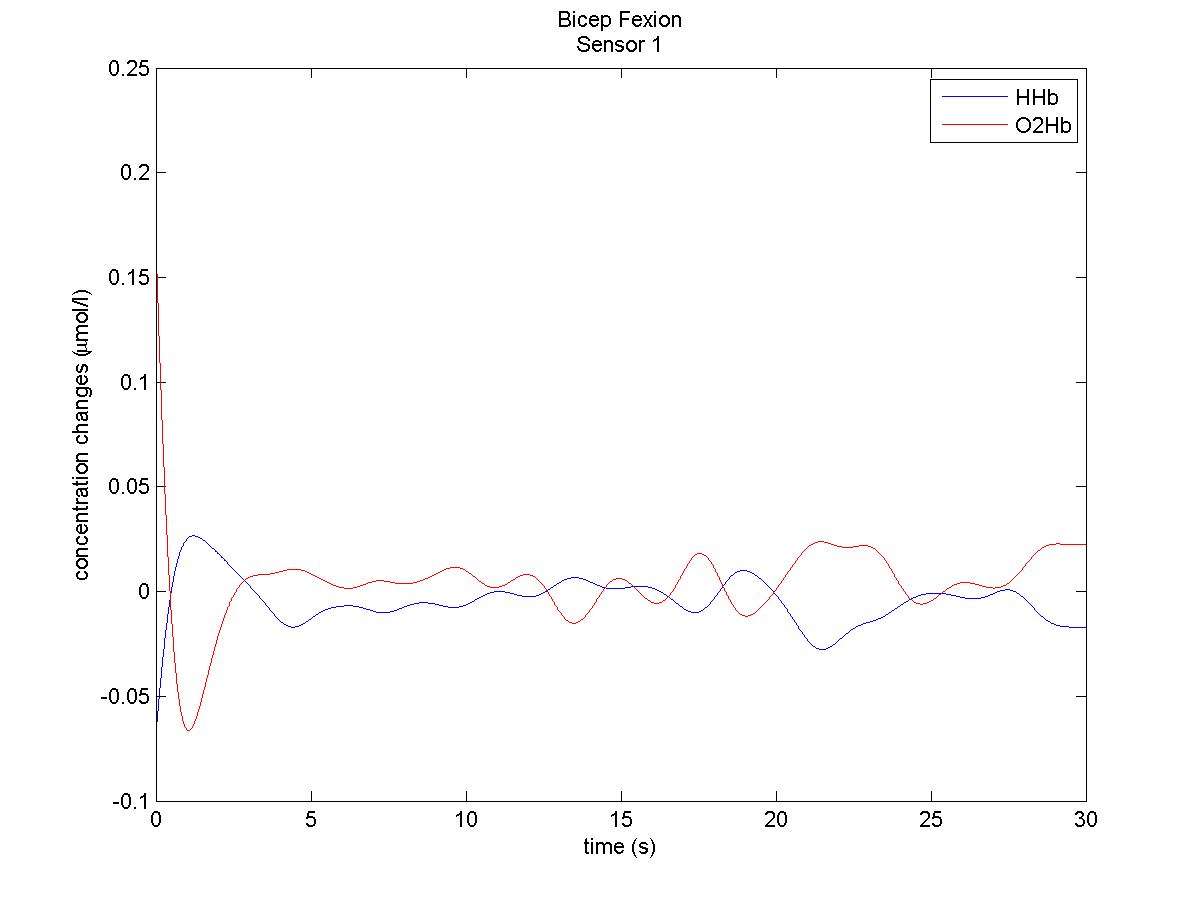
\includegraphics[width=4in]{BicepFexion/sensor1.png}}
\subfigure[Sensor 2]{ 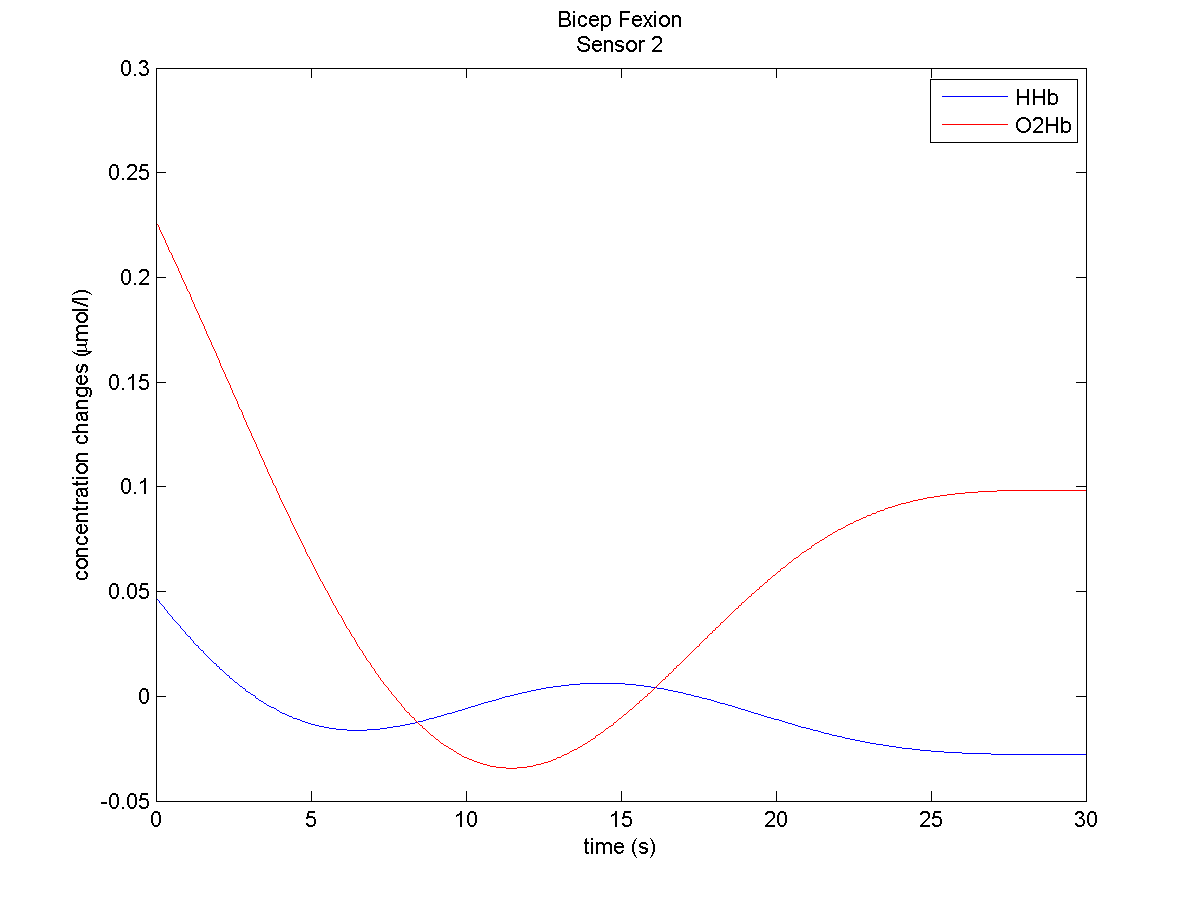
\includegraphics[width=4in]{BicepFexion/sensor2.png}}
\caption[Bicep Measurements with Continuous Flexion and Extension]{The result of having the subject continually flex and extend their bicep with the sensor placed over the bicep under activity. The change in concentration of oxyhaemoglobin is marked in red and the change in concentration of deoxyhaemoglobin is marked in blue. The subject stopped continuously flexing and extending their arm at around 8s, leaving it in the extended state until around 15s, where they began flexing and extending their bicep again}
\end{figure}


\begin{figure}[htp]
\centering
\subfigure[Sensor 1]{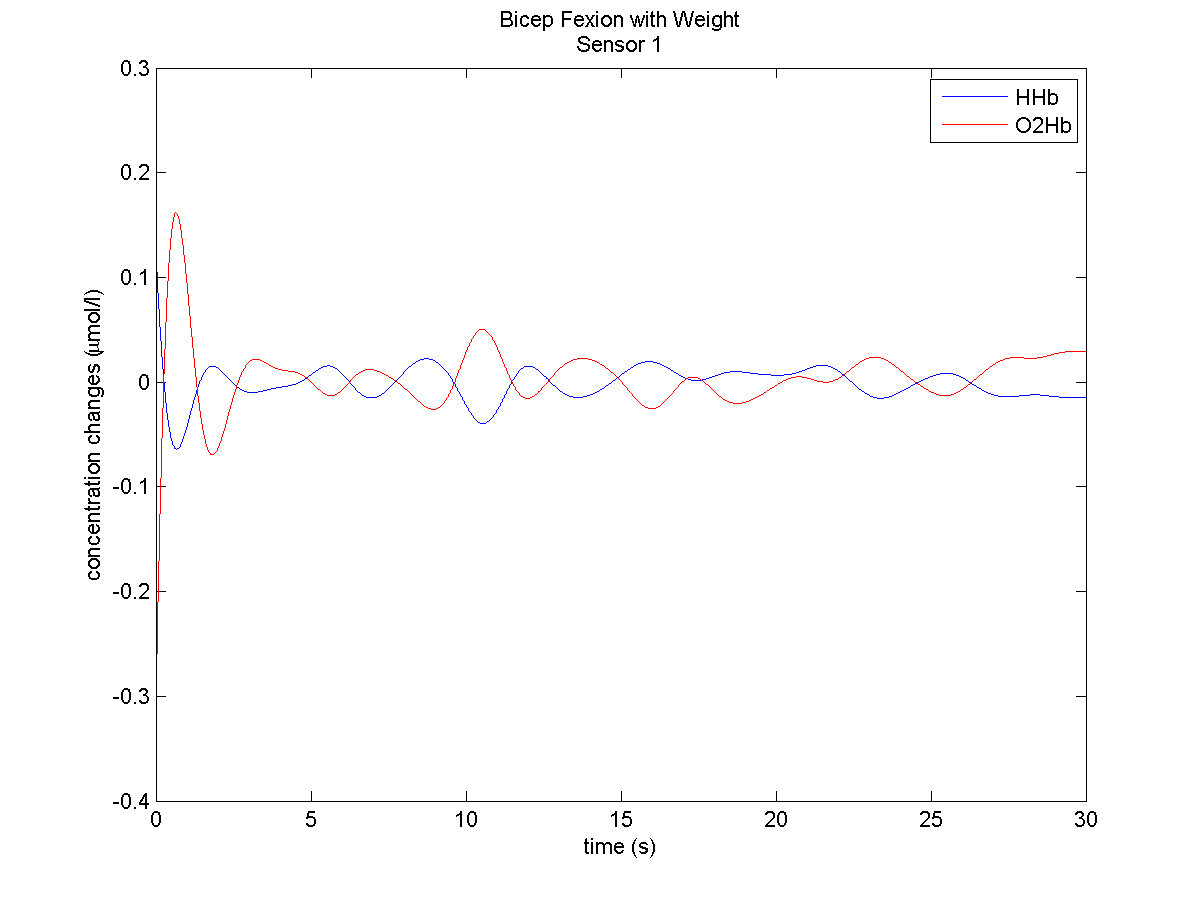
\includegraphics[width=4in]{BicepFexionWeight/sensor1.png}}
\subfigure[Sensor 2]{ 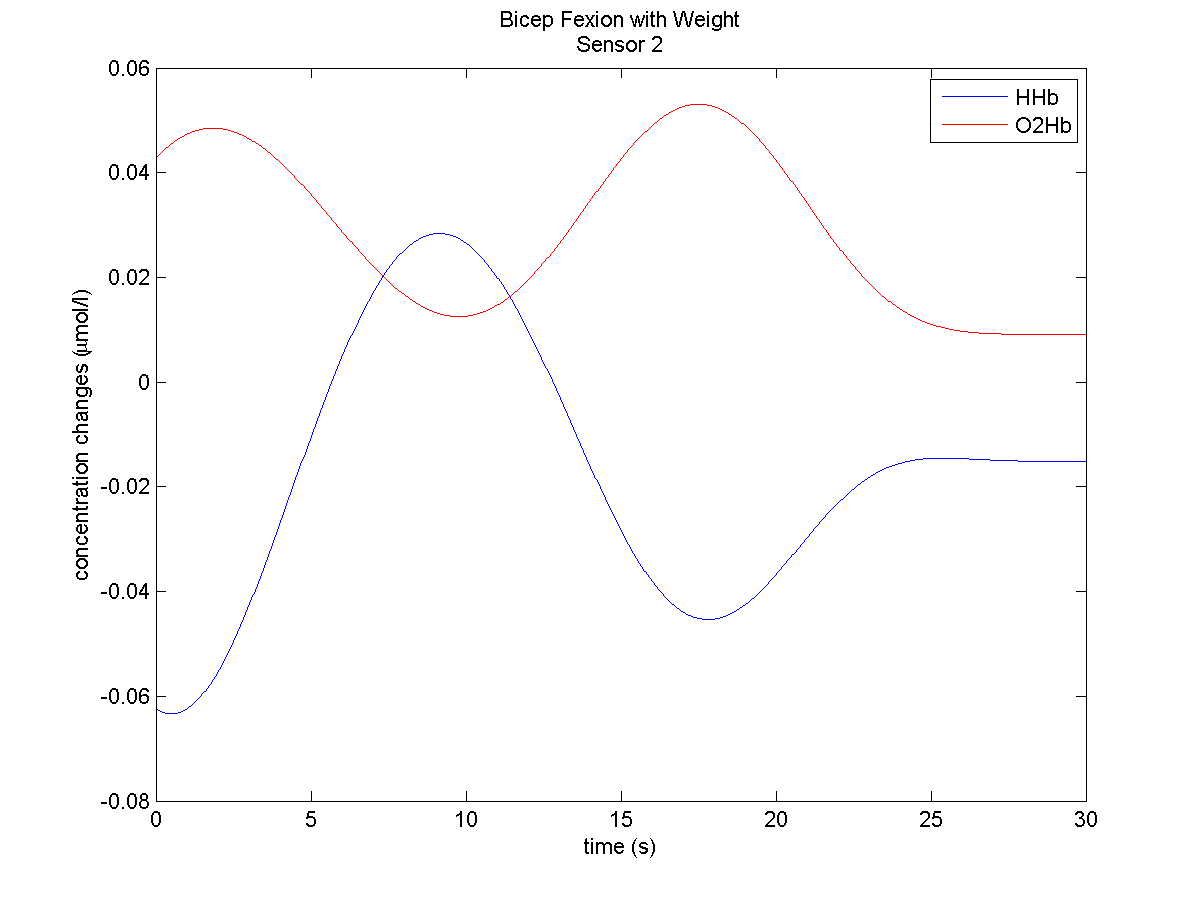
\includegraphics[width=4in]{BicepFexionWeight/sensor2.png}}
\caption[Bicep Measurements with Continuous Fexion and Extension with a Weight]{The result of having the subject continually flex and extend their bicep with a heavy weight in their hand with the sensor placed over the bicep under activity. The change in concentration of oxyhaemoglobin is marked in red and the change in concentration of deoxyhaemoglobin is marked in blue. The subject began lifting the weight at 0s, became fatigued at around 6s and was unable to lift the weight, began lifting the weight again at around 11s, finally becoming fatigued at around 23s. The subject still held the weight in their hand while fatigued, continually trying to lift it.}
\end{figure}

These results prove interesting, the system can indeed measure muscle activity. With the change in oxyhaemoglobin rates increasing during muscle activity and decreasing when not under activity, similar to brain activity. Interestingly, it can be seen that when trying to lift the wight the change in concentrations is higher than when not lifting any weight. This shows that when trying to lift more weight, the muscle has an increased need for oxygen. It can also be seen that when the muscle is fatigued, rather than having the change in oxyhaemoglobin decrease to below 0 and the change in deoxyhaemoglobin increase to above 0, the change in oxyhaemoglobin is constant and a positive value. Similarly, the change in deoxyhaemoglobin is constant and a negative value. This shows the muscle still requires oxygen and oxygenated blood is still coming in trying to restore the muscle to normal, while the muscle fibres are constantly consuming oxygen.

\section{Remarks}

This system is far from perfect. Every couple of measurements will result in one bad one that is either riddled with noise or does not make any sense. However, repeating the same measurement later on may yield positive results. It has not been determined what causes this. When the results are positive, they are repeatable, though.

The system has very good battery life. Granted it is powered by three AA batteries. Throughout the entire prototyping phase, the batteries were never needed to be changed. Previous systems have shown to have a battery life of just 3 hours \cite{rosen05}. The exact battery life of the system when constantly on is unknown, it should compete favourably with those previous systems though. The system has a ridiculously long standby time, having been in standby for at least 24hours. This is all due to the low power components in the system. 

While the prototype is not portable by all definitions of the word, it is battery powered and wireless and can be easy transported for use in the field. Due to the use of the breadboard the prototype is fairly large. However, should a PCB be made for the system, it could easily be made to be 6cm by 2cm, excluding the USB to UART module. At this size, the system wold definitely be portable by all definitions of the word. 